\begin{figure}
\quad 1.\quad В ходе работы с виртуальной машиной у меня возникла необходимость перенести её с одного своего устройства на другое.
\newline Для этого я открыл Virtual Box, нажал правой кнопкой мыши по своей виртуальной машине и выбрал пункт клонировать. В появившемся окне я указал имя нового клона и его путь по которому он будет сохранён. Так же в графе «Политика MAC-адреса» выбрал вариант: «Сгенерировать новые MAC-адреса всех сетевых адаптеров».

		\centering
		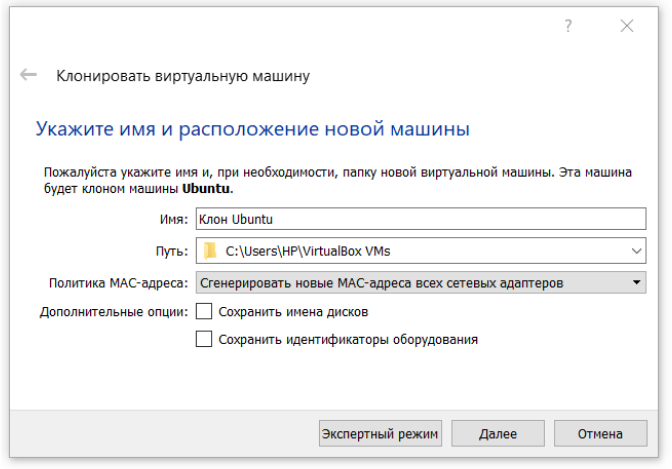
\includegraphics[width=0.6\linewidth]{img/8.png}
\caption{Окно клонирования.}
\label{ris:image}
\end{figure}

\begin{figure}
\quad В следующем окне нужно было указать тип клонирования: полное или связное. При связном клонировании будет создана новая машина, использующая файлы виртуальных жёстких дисков клонируемой машины и нельзя перенести её на другой компьютер без переноса клонируемой. При полном клонировании, будет создана полная копия клонируемой виртуальной машины (включая все файлы виртуальных жёстких дисков). Поэтому я выбрал полное клонирование.
\end{figure}

\begin{figure}
\quad В окне с указанием цели клонирования, я указал клонировать всё, чтобы новая машина не только отражала текущее состояние клонируемой машины, но и имела копии всех снимков её древа снимков.
\end{figure}

\begin{figure}
\quad Далее я нажал на кнопку «клонировать», после чего и запустился процесс клонирования. По его завершению я перенёс новую машину на флэшку. Это можно сделать нажав в Virtual Box на клон правой кнопкой мыши и выбрать пункт «Переместить». Или просто зайти в папку, в которую был сохранён наш клон, и переместить его уже оттуда.
\end{figure}

\begin{figure}
\quad Далее я подсоединил флэшку к другому компьютеру и перенёс машину в папку Virtual Box. Открыв Virtual Box, я нажал вверху на кнопку «Машина» и выбрал пункт добавить. После чего я нашёл свою машину и нажал кнопку «Открыть».

		\centering
		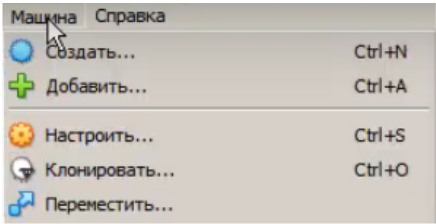
\includegraphics[width=0.4\linewidth]{img/9.png}
\caption{Добавление виртуальной машины.}
\label{ris:image}
\end{figure}

\begin{figure}
\quad Виртуальная машина добавлена. Но зайдя в настройки, то можно увидеть, что объём выделенной основной памяти составляет всего лишь 2 гигабайта, что слишком мало для работы с машиной. Так как наша машина находится в состоянии «Сохранена», мы не можем изменять её настройки. Поэтому я нажал правой кнопкой мыши по перенесённому клону, и выбрал пункт «Сбросить сохранённое состояние». После чего я снова нажал правой кнопкой мыши по машине, выбрал пункт «Настроить…» и в «Системе» выделил нужное количество памяти.

		\centering
		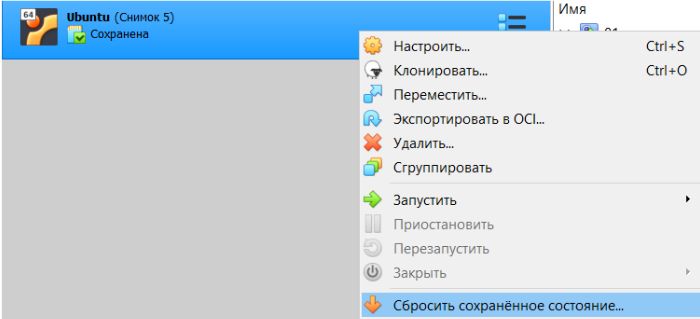
\includegraphics[width=0.65\linewidth]{img/10.png}
\caption{Настройка памяти.}
\label{ris:image}
\end{figure}

\begin{figure}
\quad Далее я также зашёл в «Носители» и выбрал свой жёсткий диск, так как иначе при запуске виртуальной машины мы бы ничего не увидели.

		\centering
		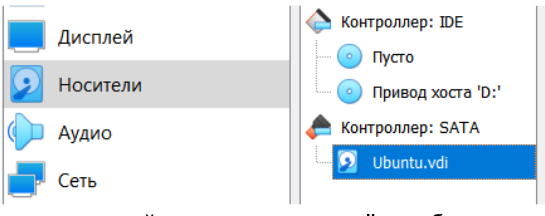
\includegraphics[width=0.65\linewidth]{img/11.png}
\caption{Настройки. Носители.}
\label{ris:image}

\end{figure}

\begin{figure}
\quad Теперь клон виртуальной машины перемещён, добавлен на новый компьютер и с ним можно работать.
\end{figure}

\begin{figure}
\quad Есть и альтернативный способ переноса виртуальной машины с одного устройства на другое, с помощью функций «Экспорт» и «Импорт».
\end{figure}

\begin{figure}
\centering
Экспорт виртуальной машины
\label{ris:image}
\end{figure}

\begin{figure}
\quad Экспорт конфигурации виртуальной машины происходит в файл формата .ova (Open Virtual Appliance). Это универсальный формат для хранения данных виртуальной машины, файлы .ova могут использоваться в разных программах виртуализации: VirtualBox, VMware Workstation, Microsoft Hyper-V. Виртуальная машина, экспортированная в файл .ova, затем может быть импортирована как в VirtualBox, так и в VMware Workstation, Microsoft Hyper-V.
\end{figure}

\begin{figure}
\quad В меню программы нужно зайти в «Файл» и выбрать пункт «Экспорт конфигураций». В открывшемся окне выбираем машину для экспорта, и нажимаем «Далее».

		\centering
		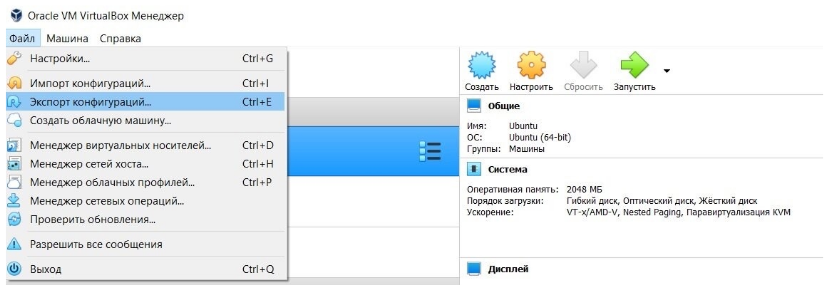
\includegraphics[width=0.65\linewidth]{img/12.png}
\caption{«Экспорт конфигураций».}
\label{ris:image}

\end{figure}

\begin{figure}
\quad Выбираем место размещения после экспорта. Также лучше выбрать «Включать МАС-адреса всех сетевых адаптеров», нажимаем «Далее».

		\centering
		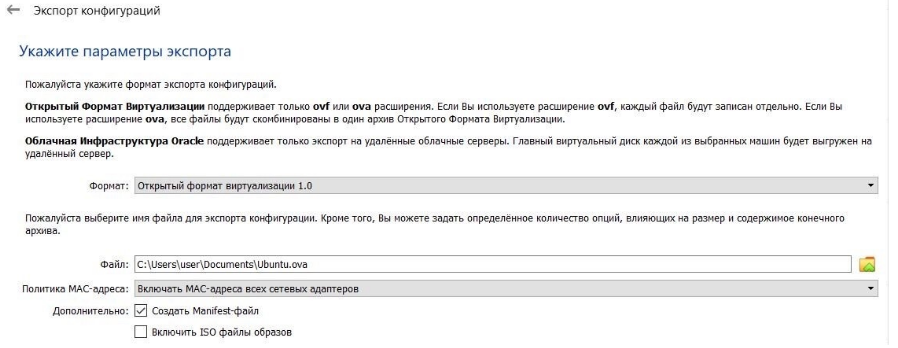
\includegraphics[width=0.65\linewidth]{img/13.png}
\caption{МАС-адреса сетевых адаптеров.}
\label{ris:image}

\end{figure}

\begin{figure}
\quad В следующем окне оставляем без изменений, и нажимаем “Экспорт”. Сам экспорт занимает несколько минут, в зависимости от размера виртуальной машины. После экспорта в указанном месте создается файл.
\end{figure}

\begin{figure}
\centering
Импорт виртуальной машины
\label{ris:image}
\end{figure}

\begin{figure}
\quad Теперь необходимо скопировать файл на флэшку. Далее на втором компьютере заходим в программу Virtual Box и нажимаем вверху «Файл» и выбираем пункт «Импорт конфигураций».

\centering
		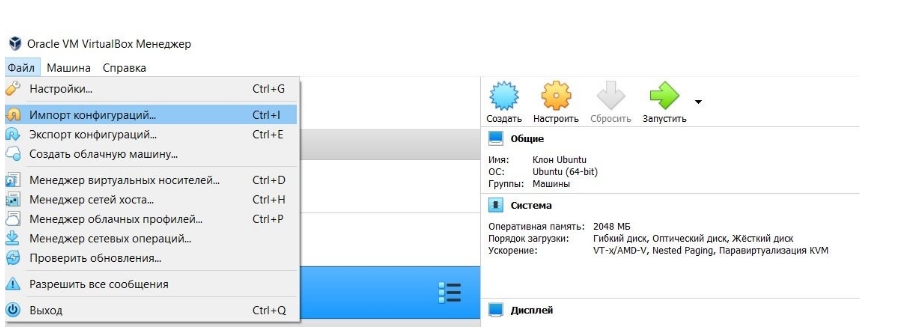
\includegraphics[width=0.65\linewidth]{img/14.png}
\caption{Импорт конфигураций.}
\label{ris:image}
\end{figure}

\begin{figure}
\quadВ окне импорта выбираем место размещения файла виртуальной машины, нажимаем «Далее». В следующем окне можно изменить параметры импорта, например, увеличить количество процессоров. Также желательно «Включать (сгенерировать новые) МАС-адреса всех сетевых адаптеров», и нажимаем «Импорт».
\end{figure}

\begin{figure}
\quad Импорт также в зависимости от размера виртуальной машины может занимать несколько.
\end{figure}

\begin{figure}
\quad После импорта виртуальная машина появляется в списке и с ней уже можно будет работать.
\end{figure}

